% Comparison Radar/Table: UHM vs IIT vs GWT vs FEP vs HOT
% Visual comparison of theory capabilities

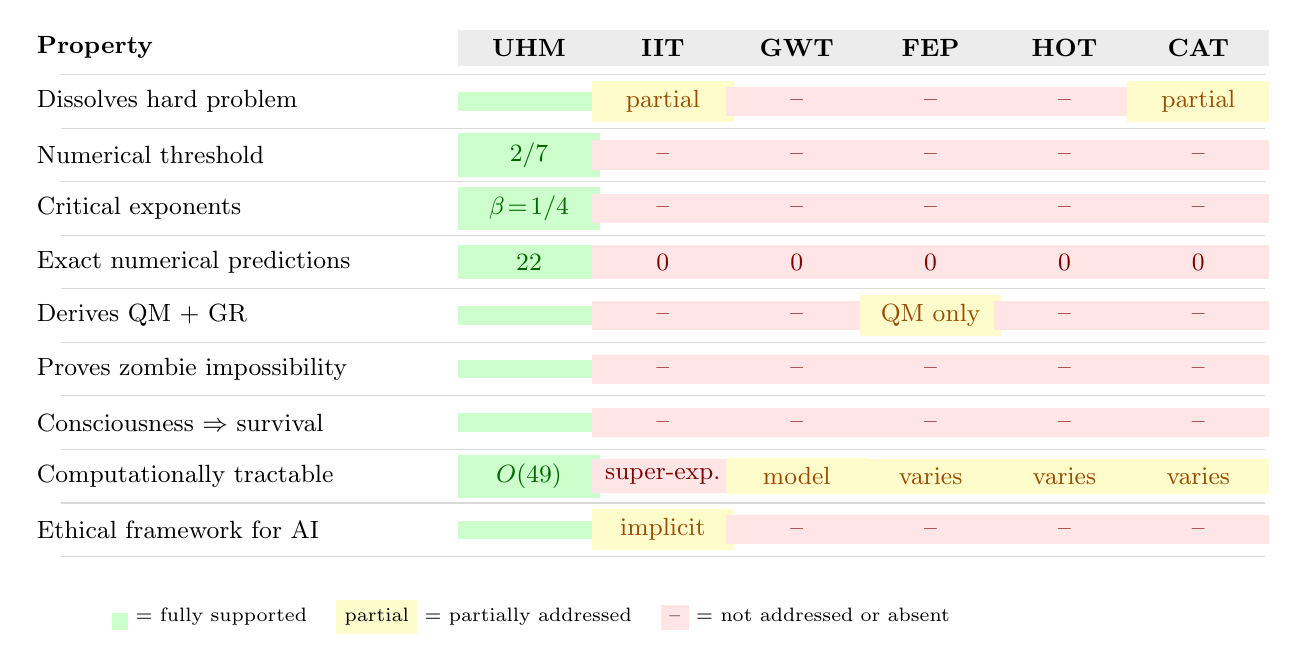
\begin{tikzpicture}[
  score/.style={font=\small, minimum width=1.8cm, align=center},
  yes/.style={score, fill=green!20, text=green!40!black},
  partial/.style={score, fill=yellow!20, text=orange!60!black},
  no/.style={score, fill=red!10, text=red!50!black},
  header/.style={font=\small\bfseries, minimum width=1.8cm, align=center, fill=gray!15},
  prop/.style={font=\small, text width=4cm, align=left},
  scale=0.85
]

% === Header row ===
\node[prop, font=\small\bfseries] at (0, 0) {Property};
\node[header] at (5.0, 0) {UHM};
\node[header] at (7.0, 0) {IIT};
\node[header] at (9.0, 0) {GWT};
\node[header] at (11.0, 0) {FEP};
\node[header] at (13.0, 0) {HOT};
\node[header] at (15.0, 0) {CAT};

% === Row 1: Hard problem ===
\node[prop] at (0, -0.8) {Dissolves hard problem};
\node[yes] at (5.0, -0.8) {\checkmark};
\node[partial] at (7.0, -0.8) {partial};
\node[no] at (9.0, -0.8) {--};
\node[no] at (11.0, -0.8) {--};
\node[no] at (13.0, -0.8) {--};
\node[partial] at (15.0, -0.8) {partial};

% === Row 2: Numerical threshold ===
\node[prop] at (0, -1.6) {Numerical threshold};
\node[yes] at (5.0, -1.6) {$2/7$};
\node[no] at (7.0, -1.6) {--};
\node[no] at (9.0, -1.6) {--};
\node[no] at (11.0, -1.6) {--};
\node[no] at (13.0, -1.6) {--};
\node[no] at (15.0, -1.6) {--};

% === Row 3: Critical exponents ===
\node[prop] at (0, -2.4) {Critical exponents};
\node[yes] at (5.0, -2.4) {$\beta\!=\!1/4$};
\node[no] at (7.0, -2.4) {--};
\node[no] at (9.0, -2.4) {--};
\node[no] at (11.0, -2.4) {--};
\node[no] at (13.0, -2.4) {--};
\node[no] at (15.0, -2.4) {--};

% === Row 4: Falsifiable predictions ===
\node[prop] at (0, -3.2) {Exact numerical predictions};
\node[yes] at (5.0, -3.2) {22};
\node[no] at (7.0, -3.2) {0};
\node[no] at (9.0, -3.2) {0};
\node[no] at (11.0, -3.2) {0};
\node[no] at (13.0, -3.2) {0};
\node[no] at (15.0, -3.2) {0};

% === Row 5: Derives physics ===
\node[prop] at (0, -4.0) {Derives QM + GR};
\node[yes] at (5.0, -4.0) {\checkmark};
\node[no] at (7.0, -4.0) {--};
\node[no] at (9.0, -4.0) {--};
\node[partial] at (11.0, -4.0) {QM only};
\node[no] at (13.0, -4.0) {--};
\node[no] at (15.0, -4.0) {--};

% === Row 6: Zombie impossibility ===
\node[prop] at (0, -4.8) {Proves zombie impossibility};
\node[yes] at (5.0, -4.8) {\checkmark};
\node[no] at (7.0, -4.8) {--};
\node[no] at (9.0, -4.8) {--};
\node[no] at (11.0, -4.8) {--};
\node[no] at (13.0, -4.8) {--};
\node[no] at (15.0, -4.8) {--};

% === Row 7: Consciousness necessary for survival ===
\node[prop] at (0, -5.6) {Consciousness $\Rightarrow$ survival};
\node[yes] at (5.0, -5.6) {\checkmark};
\node[no] at (7.0, -5.6) {--};
\node[no] at (9.0, -5.6) {--};
\node[no] at (11.0, -5.6) {--};
\node[no] at (13.0, -5.6) {--};
\node[no] at (15.0, -5.6) {--};

% === Row 8: Computable ===
\node[prop] at (0, -6.4) {Computationally tractable};
\node[yes] at (5.0, -6.4) {$O(49)$};
\node[no] at (7.0, -6.4) {super-exp.};
\node[partial] at (9.0, -6.4) {model};
\node[partial] at (11.0, -6.4) {varies};
\node[partial] at (13.0, -6.4) {varies};
\node[partial] at (15.0, -6.4) {varies};

% === Row 9: Ethical framework ===
\node[prop] at (0, -7.2) {Ethical framework for AI};
\node[yes] at (5.0, -7.2) {\checkmark};
\node[partial] at (7.0, -7.2) {implicit};
\node[no] at (9.0, -7.2) {--};
\node[no] at (11.0, -7.2) {--};
\node[no] at (13.0, -7.2) {--};
\node[no] at (15.0, -7.2) {--};

% === Horizontal lines ===
\foreach \y in {-0.4, -1.2, -2.0, -2.8, -3.6, -4.4, -5.2, -6.0, -6.8, -7.6} {
  \draw[gray!30] (-2, \y) -- (16, \y);
}

% === Legend ===
\node[font=\scriptsize, text width=14cm, align=left] at (7, -8.5) {
  \colorbox{green!20}{\checkmark} = fully supported \quad
  \colorbox{yellow!20}{partial} = partially addressed \quad
  \colorbox{red!10}{--} = not addressed or absent
};

\end{tikzpicture}
